\documentclass[__main__.tex]{subfiles}

\begin{document}

\qtitle{К}{21}
Временное и стационарное уравнения Шрёдингера. Электрон в бесконечно глубокой одномерной потенциальной яме.\\

\begin{definition}
    Временное уравнение Шредингера:
    \begin{gather}
        i\hbar\frac{\partial{}}{\partial{t}}\Psi = \hat{H}\Psi,
        \llabel{shred-time}
    \end{gather}
    где $\hat{H}$ - гамильтониан.
\end{definition}
\begin{definition}
    Стационарное уравнение Шредингера:
    \begin{gather}
        \hat{H}\psi(\vec{r})=\varepsilon\psi(\vec{r}),
        \llabel{shred-stac}
    \end{gather}
    где $\hat{H}=\frac{\hat{p}}{2m}+U(t,\vec{r})$ - гамильтониан или оператор полной энергии, $\psi(\vec{r})$ - волновая функция, $\varepsilon$ - некая константа,  отвечающая собственным значениям оператора полной энергии.
\end{definition}
\begin{definition}
    \textbf{Потенциальная яма} – ограниченная область пространства с пониженной потенциальной энергией частицы.
    \llabel{hole}
\end{definition}
\begin{wrapfigure}{L}{.3\linewidth}
    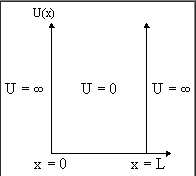
\includegraphics{k-21-1}
    \caption{Бесконечная прямоугольная потенциальная яма}
    \llabel{k-21-hole}
\end{wrapfigure}
Итак, пусть частица массы $m$ находится в одномерной потенциальной яме бесконечной глубины (\lref{k-21-hole}).Потенциальная энергия $U$ удовлетворяет следующим граничным условиям:
\begin{gather}
    \llabel{k-21-boundary}
    U(x)=
    \begin{cases}
        \infty & x<0,x>L,       \\
        0      & 0\leq x \leq L \\
    \end{cases}.
\end{gather}
При таких граничных условиях частица находится внутри потенциальной ямы $0 < x < L$ и не может выйти за ее пределы, т.е.
\begin{gather}
    \llabel{k-21-psi}
    \Psi(x)=0\hspace{0.5cm}x<0,x>L
\end{gather}
Используя стационарное уравнение Шредингера для случая $U=0$, получим
\begin{gather}
    \llabel{k-21-shredforzero}
    \frac{d^2\Psi}{dx^2}+\frac{2mE}{\hbar^2}\Psi=0
\end{gather}
Уравнение \lref{k-21-shredforzero} описывает положение частицы внутри потенциальной ямы. \\
Для бесконечной одномерной потенциальной ямы имеем следующее:
\begin{enumerate}
    \item Энергия частицы принимает определенные дискретные значения. Обычно говорят, что частица находится в определенных энергетических состояниях.
          \begin{gather}
              E_n=\frac{n^2\mathcal{\pi}^2\hbar^2}{2mL^2}, \hspace{0.5cm} n=1,2,3...
          \end{gather}
    \item Частица может находиться в каком-то одном из множества энергетических состояний.
    \item Частица не может иметь энергию равную нулю.
    \item Каждому значению энергии $E_n$ соответствует собственная волновая функция $\Psi_n$, описывающая данное состояние.
    \item Для собственной функции $\Psi_1(x)$ вероятность обнаружить частицу в точке x = L/2 максимальна. Для состояния $\Psi_2(x)$ вероятность обнаружения частицы в этой точке равна 0 и т.д.
\end{enumerate}

\end{document}